create functions which map inputs to desired outputs
\begin{itemize}
    \item Regression: find output value based on input. Example: given a house has 5 bedrooms, 1000 square meters, what is its price?
    \item Classification: assign element to a group. Example: the first mushroom is edible, the second is not.
\end{itemize}

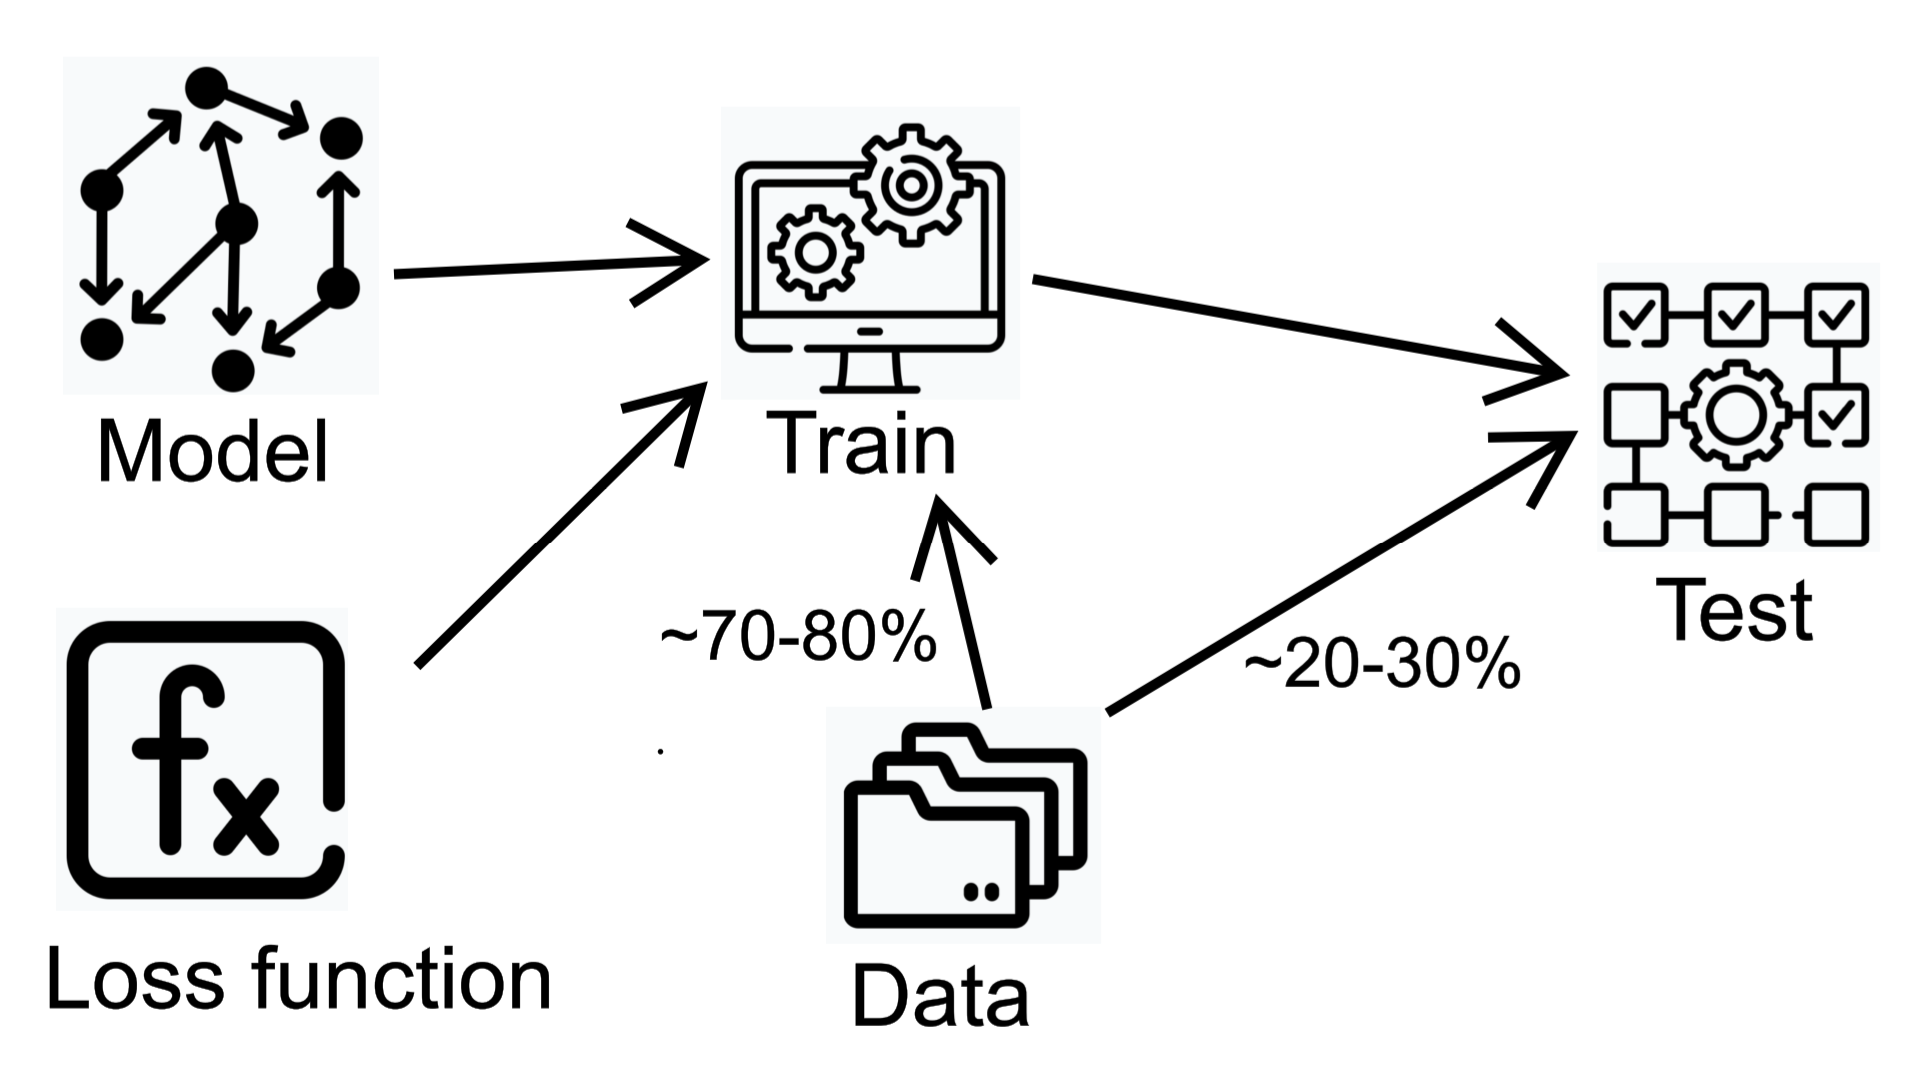
\includegraphics[width = \linewidth]{src/8_ml/images/ml_overview.png}

Models:
\begin{itemize}
    \item Decision tree classifier
    \item Linear Regression $y = w_1 x_1 + w_2 x_2 +...+ w_n x_n$
    \item Neural Network and activation function (Sigmoid, Relu, Tanh)
\end{itemize}

Loss function:
\begin{itemize}
    \item $\frac{\text{\# wrongly classified examples}}{\text{\# total examples}}$
    \item Mean Square Error
    \item L2 (Gauss Loss)
\end{itemize}

Test:
\begin{itemize}
    \item R2-Score $1 - \frac{MSE(D, f)}{MSE(D, f_0)}, f_0 = \frac{1}{n} \sum_{i = 0}^{n} y_i$
\end{itemize}